\documentclass[12pt, a4paper]{article}
\usepackage[UTF8]{ctex}
\usepackage{amsmath}
\usepackage{amssymb}
\usepackage{amsthm}
\usepackage{geometry}
\usepackage{enumitem}
\usepackage{indentfirst}
\usepackage{caption}
\usepackage{fancyhdr}
\usepackage{booktabs}
\usepackage{titlesec}
\usepackage{draftwatermark}
\usepackage{graphicx} % 导入图像的宏包、单图





% 页面布局设置
\geometry{top=2.54cm, bottom=2.54cm, left=3.18cm, right=3.18cm}

% 行距设置
\linespread{1.5}

%设置水印
\SetWatermarkText{B站：布加拉提}
\SetWatermarkScale{0.4}
% 段落设置
\setlength{\parindent}{2em}
\setlength{\parskip}{0.5em}

% 节标题格式设置
\titleformat{\section}{\normalfont\Large\bfseries}{第\chinese{section}章、}{1em}{}
\titlespacing{\section}{0pt}{2.5ex plus 1ex minus .2ex}{1.3ex plus .2ex}

% 定理环境设置
\newtheoremstyle{solution}
{}
{}
{}
{}
{\bfseries}
{、}
{1em}
{}
\theoremstyle{solution}
\newtheorem{sol}{解}

% 页眉页脚设置
\pagestyle{fancy}
\fancyhf{}
\fancyhead[C]{b站布加拉提整理（回忆版）b站甘茶w独家讲解}
\fancyfoot[C]{\thepage}

\rfoot{整理人：八方\\资源提供：考研乔瑟夫}
\lhead{
\includegraphics[width=0.06\linewidth]{p1.png}}
\rhead{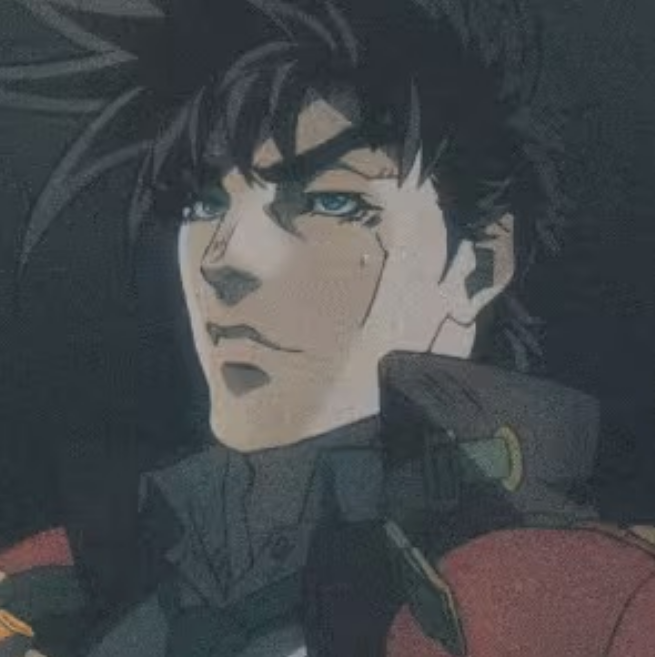
\includegraphics[width=0.06\linewidth]{p2.png}}
\renewcommand{\headrulewidth}{0.4pt}
\renewcommand{\footrulewidth}{0.4pt}

\begin{document}

\begin{center}
\Large\textbf{2005哈工大硕士考试试题：805物理光学}
\end{center}




\section*{一、填空（每空2分，共32分）}
\begin{enumerate}
    \item 在迈克尔逊干涉仪的一支光路中，垂直于光路放入折射率为n的透明介质薄膜后，测出两光来的光程差的改变量为一个波长$\lambda$。则膜的厚度是\_\_\_\_\_.
    \item (重复)波长为\(\lambda\)的单色平行光垂直入射到一狭缝上，若第一级暗纹的位置对应的衍射角为$\theta=±\pi/6$,则缝宽的大小为\_\_\_\_\_.
    \item 复色波的群速度定义为\_\_\_\_\_.它与相速度的关系为\_\_\_\_\_.
    \item 夫琅和费多缝衍射主级大的条件\_\_\_\_\_，多缝衍射极小的条件是\_\_\_\_\_，多缝衍射主级大的角宽度为\_\_\_\_\_.
    \item 圆孔菲涅尔衍射一般用半波法进行分析，在圆孔后通过圆孔中心光轴上点的光强随着距高的改变，光强\_\_\_\_\_变化，当圆孔相对该点的半波带为\_\_\_\_\_时，光强为亮点。
    \item F-P标准具的自由光谱范围\_\_\_\_\_，分辨本领为\_\_\_\_\_.
    \item 用单色光垂直照射在观察牛顿环的装置中，当平凸透镜垂直向上缓慢平移而远离平面玻璃时，可以观察到这些环状干涉条纹\_\_\_\_\_.观察视场内条纹数\_\_\_\_\_。
    \item 在磁场作用下，使光矢量发生旋转，其磁致旋光的方向与磁场方向\_\_\_\_\_，与光的传播方向\_\_\_\_\_。利用这一特点，可通过多次反射\_\_\_\_\_磁光效应。

\end{enumerate}
\section*{二、简答题（每题5分，共30分）}
\begin{enumerate}
    \item 将一个光波分割成两个相干光波有几种方法？举例说明。
    \item 两个光波的叠加和干涉是否相同？为什么？举例说明。
    \item 对杨氏干涉实验，在观察屏的不同位置观察干涉条纹，其条纹形状与间距是否一样？
    \item 什么是部分偏振光？如何评价其偏振程度？
    \item 光波的折射遵循什么规律？什么情况下不遵循这一规律？
    \item 理想光学系统的分辨本领指的是什么？怎么可以简答确定这一本领？
\end{enumerate}
\section*{三、论述与讨论题（共35分）}
\begin{enumerate}
    \item 光矢量与入射面之夹角被称为振动地方位角，设入射的线偏振光的方位角为\(\alpha_1\),入射角为\(i_1\),折射角为\(i_2\),推到出反射线偏振光的方位角\(\alpha_2\)的表达式。若入射角为布儒斯特角，反射线偏振光的方位角为多少？
    \item 在一对正交的偏振片\(p_1\)和\(p_2\)之间插入一块\(\lambda/4\)波片，将\(\lambda/4\)波片旋转一周。会看到什么现象？说明原因。若将\(\lambda/4\)波片光轴与\(p_1\)近光轴方向成60度角，有一强度为\(I_0\)的单色自然光正入射于该系统，求出射光的强度。忽略反射，吸收损耗。要求做出示意图。
    \item 以杨氏双缝实验为例，简述光波干涉与衍射的关系。
    \item 条纹对比度是表征光场相干程度的参量，影响条纹可见度（对比度）的主要因素有哪些？简述时间相干性，空间相干性与各因素的关系。
    \item 波法线菲涅尔方程为：\\ $\frac{K_1^2}{\frac{1}{n^2}+\frac{1}{\varepsilon_1}}+\frac{K_2^2}{\frac{1}{n^2}-\frac{1}{\varepsilon_2}}+\frac{K_3^2}{\frac{1}{n^2}-\frac{1}{\varepsilon_3}}=0$\\请说明该式是如何描述晶体的光学各向异性的？

    \item 下图为检验镀有反射膜的直角棱镜的原理图。请问：    
    \begin{enumerate}
        \item 若在观察屏上看到干涉条纹，则对光源有何要求？
        \item 该干涉装置能检验直角棱镜的何项指标？此时对装置中的元件有何种要求？
        \item 叙述其工作原理。
    \end{enumerate}
    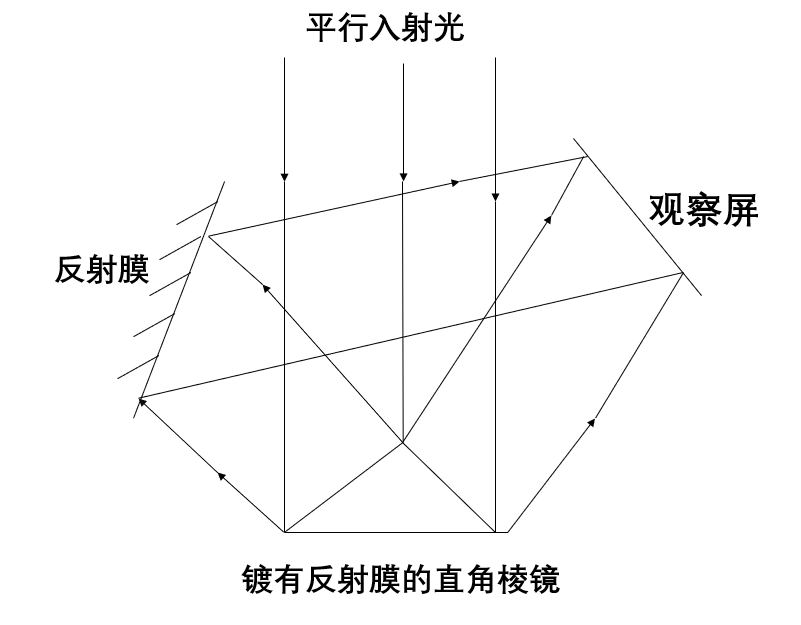
\includegraphics[width=0.7\linewidth]{05.png}

\end{enumerate}
\section*{四、计算题（共35分）}
\begin{enumerate}
    \item (重复)通过偏振片观察部分偏振光时，当偏振光绕入射光方向旋转到某一位置上，透射时光强为极大。然后再将偏振片旋转30度，发现透射光强为为极大，然后再将偏振片旋转30度发现投射光强为极大值的4/5，试求该入射部分偏振光的偏振度P及该光内自然光与线偏振光强之比。
    \item 一块光栅长150mm每毫米有1200条纹，使用的光源为钠黄光，包括两条谱线\(\lambda_1=589nm\)和\(\lambda_2=589.6nm\)，透镜的焦距为1m，求：
    \begin{enumerate}
        \item 求光束垂直入射到光栅时，一级光谱中两条谱线的间隔和半角宽度；
        \item 求波长\(\lambda=500nm\)的一级光谱白色分辨本领和自由光谱范围。
        \item 平行光垂直入射和30度角斜入射时，分别最多能观察到几级谱线？
    \end{enumerate}






\end{enumerate}
\end{document}